\chapter{Risk Analysis}
	The Risk Analysis table defines a potential set of risks that our group could face, as setbacks to timely progression towards our finished project. For each risk, there are two potential consequences, a probability value (0$\rightarrow$1), a severity value (0$\rightarrow$10), an impact value (impact=probability*severity), and two potential mitigation strategies. The risks are ordered from greatest to least impact value (top-to-bottom).

\begin{table}[]
\caption{Risk Table}
\label{riskTable}
\begin{tabular}{l}
    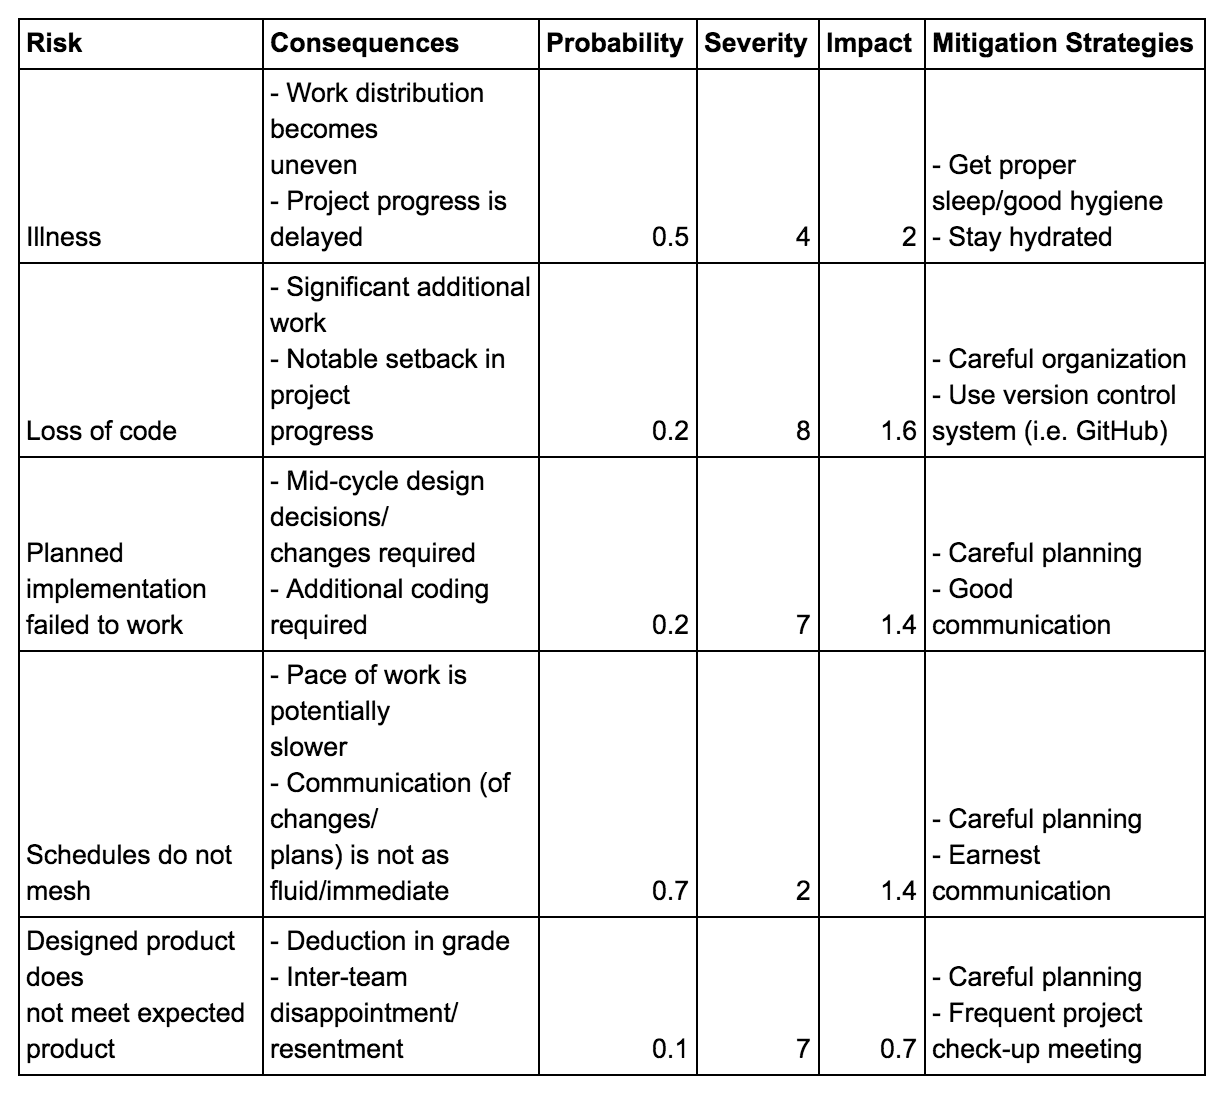
\includegraphics[scale = 0.8]{riskTable.png}
\end{tabular}
\end{table}